\chapter{Literature Review}
\label{chap:LiteratureReview}
This chapter reviews key literature that forms the theoretical foundation of this research. Specifically, the $n$-gram language model, fuzzy clustering, and Fourier transforms will be discussed. Additionally, specific details of these topics will be examined to demonstrate their practical applications within this project.

\noindent Relevant definitions and properties needed to understand these applications will be introduced, alongside examples and comparisons to provide a more comprehensive and nuanced understanding of the theory.

\section{n-gram language model}
The $n$-gram language model analyzes a sequence of symbols by examining sets of frames, known as $n$-grams. This model is designed to construct a natural language model based on the assumption that each new symbol is statistically influenced by the preceding symbols. For example, the phrase '\texttt{I am playing }' could be followed by '\texttt{a piano}' or '\texttt{with a dog}'. The $n$-gram model assumes that the continuation of this phrase depends solely on a finite window of preceding words or characters, and assigns '\texttt{a piano}' a certain probability of being the most natural continuation. However, as language modeling techniques have advanced, the $n$-gram model has largely been replaced by more sophisticated models, such as transformers\footnote{For more information on transformers, see \url{https://en.wikipedia.org/wiki/Transformer_(deep_learning_architecture)}}.

\begin{figure}[ht]
	\centering
	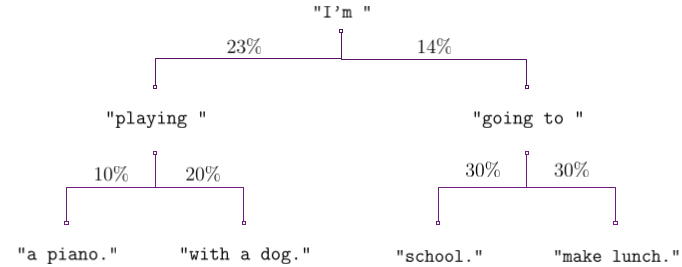
\includegraphics[width=\linewidth]{Figures/exngrammodel.png}
\end{figure}

\noindent The $n$-gram language model, first introduced by Shannon and described in \citet{Shannon_ngrammodel}, was later applied in \citet{SapAttribution} for the purpose of author attribution. In this case, the goal was not to generate natural text but to identify the author of a given text. The research found that the best performance was achieved using $8$-grams, and attribution was done by comparing each known author's work with the target text.

\noindent An additional development of this model extended its use to a completely different field: images. In the research thesis \cite{thesis}, this attribution method was employed to determine the authorship of a manuscript by treating the grams as square pixel tiles.

\subsection{Insights}
As previously mentioned, the $n$-gram model predicts the next characters or words to be placed based on the preceding ones. For example, if the focus is on sequences of $n$ printable characters, the model is trained on a dataset of text files, empirically deriving the probabilities $\mathbb{P}\left[w_n|w_1,\dots,w_{n-1}\right]$, where $w_i$ represents the $i$-th character of the $n$-gram.

\begin{toReview}
	\noindent In this way, a machine can construct a sentence from a few characters: $w_1,\ldots,w_{n-1}$. The algorithm iteratively selects the most probable next character $w_{n}$ given the current window of $n-1$ characters, then updates the window to $w_2,\ldots,w_{n}$ to predict $w_{n+1}$, and so on. This step-by-step process resembles a Markov chain, where each state corresponds to the current sequence of characters, and transitions between states occur with probabilities derived from the dataset.
\end{toReview}

\begin{modified}
\noindent The model assumes that the next character  depends only by the last $n-1$ characters so:
\begin{equation}
	\mathbb{P}\left[w_{n+k}|w_k\dots w_{n+k-1}\right] = \mathbb{P}\left[w_{n+k}|w_{k+1}\dots w_{n+k-1}\right] \quad \forall k
	\label{eq:ngram_model}
\end{equation}
\end{modified}
From this assumption we derive the following property:
\begin{proposition}
	\begin{modified}
		Let $w_1,\dots,w_{n-1},w_n\dots,w_{n+k}$ be a sequence of characters, where $n$ represents the size of the $n$-gram window used by the model. Specifically, the model assumes that the probability of the $n$-th character depends only on the preceding $n-1$ characters for all $n$-grams. We have that:
	\end{modified}
\begin{equation}
	\mathbb{P}\left[w_n,\dots,w_{n+k}|w_1,\dots,w_{n-1}\right] = \prod_{i=0}^{k}\mathbb{P}\left[w_{n+i}|w_{i+1}\dots w_{n+i-1}\right]
	\label{eq:ngram_model_prop}
\end{equation}
\end{proposition}

\begin{proof}
	This property is proved by using Bayes' theorem and the assumption of the model \cref{eq:ngram_model}:
\begin{align*}
	\mathbb{P}\left[w_n,\dots,w_{n+k}|w_1,\dots,w_{n-1}\right] &= \prod_{i=0}^{k}\mathbb{P}\left[w_{n+i}|w_1\dots w_{n+i-1}\right] \\
	&= \prod_{i=0}^{k}\mathbb{P}\left[w_{n+i}|w_{i+1}\dots w_{n+i-1}\right]
\end{align*}
\end{proof}

\noindent The model is built on the assumption that considering $n$-grams larger than $n$ is unnecessary. However, this limitation can introduce significant weaknesses in natural language processing, as it ignores information outside the $n$-character window. For instance, in a mystery novel, understanding the entire plot and its intricate details is crucial, something the model might overlook. Despite this, the $n$-gram model can still be quite effective in simpler contexts like everyday conversation. For example, after the input '\texttt{Hi! How are }', the model might predict '\texttt{you?}' as a natural continuation.

\noindent As mentioned earlier, this model was repurposed for a different goal by \citet{SapAttribution}. While the $n$-gram model might struggle to generate fully coherent natural language without encountering semantic inconsistencies or syntactic errors, it remains useful for capturing an author's writing style. This is achieved by training the model exclusively on texts by that author. The approach is to extract all $n$-grams from the target work and compare their distribution to that of known works by other authors. The proposed formula for comparing work $A$ with work $B$ is as follows:
\begin{equation}
	d(A,B) = \frac{1}{|D_A|+|D_B|}\sum_x\left(\frac{f_A(x)-f_B(x)}{f_A(x)+f_B(x)}\right)^2
	\label{eq:SapAttribution_dist}
\end{equation}
where $f_A(x)$ represents the frequency of the $n$-gram $x$ in the work $A$ and $|D_A|$ is the variety of observed $n$-grams.

\noindent As highlighted in \cite{thesis}, two relevant properties of this method of comparing distributions can be mentioned:
\begin{itemize}
	\item Each addendum of the summation takes on a value between $0$ and $1$.
	\item The external factor not only normalises the result so that it remains between $0$ and $1$, but also calls up the Jaccard index\footnote{For more about Jaccard index, see \url{https://en.wikipedia.org/wiki/Jaccard_index}}, improving the arithmetic mean of the summation:
	\[
		\frac{1}{|D_A|+|D_B|} = (1+J_{D_A,D_B})^{-1}\frac{1}{|D_A\cup D_B|}
	\]
	\begin{toReview}
		\noindent where $J_{D_A,D_B} := \frac{\left|D_A\cap D_B\right|}{\left|D_A\cup D_B\right|}$.

		\noindent In this way, we can see the comparison formula as a product between two types of index:
		\[
			d(A,B)=(1+J_{D_A, D_B})^{-1} \times \frac{1}{\left|D_A\cup D_B\right|}\sum_{x\in D_A\cup D_B}\left(\frac{f_A(x)-f_B(x)}{f_A(x)+f_B(x)}\right)^2
		\]
	\end{toReview}
\end{itemize}

\subsection{Implications}
We conclude this section by discussing the implications of this theory. As seen in \cref{eq:ngram_model}, no distinction is made between one $n$-gram and another. This is because $n$-grams of length 3, or slightly longer, are typically used, which are insufficient to cover a full word. However, when using $7$-grams, it becomes possible to consider the relationships between synonyms and distances between $n$-grams. For instance, we would expect some level of correlation between ‘\texttt{paper}’ and ‘\texttt{article}’ as they are synonyms.

\noindent In written texts, this rarely impacts the outcome, as there are relatively few synonyms for each term within the full vocabulary, and especially few long chains of synonyms. For example, it is unlikely that many synonyms for ‘\texttt{paper}’ begin with the string ‘\texttt{p}’ or ‘\texttt{pe}’.

\noindent As noted in \cite{thesis}, the research deliberately set appropriate image \textit{resolution} and \textit{posterization} to avoid discussions about the similarity between tiles. By controlling these parameters, the focus remained on the attribution process rather than getting lost in complex considerations of tile ‘synonyms’ and their potential concatenations.

\bigskip
We further examine the properties of the comparison formula defined in  \cref{eq:SapAttribution_dist}, particularly focusing on the problem of sparsity in $n$-grams.

\noindent Let $N$ represent the samples drawn from two absolutely continuous distributions $\mathcal{A}$ and $\mathcal{B}$ defined on $\mathbb{R}$. We partition $\mathbb{R}$ into intervals (boxes) of amplitude $1 \; / \; C$, thus transforming the original distributions into their discretized versions, $\mathcal{A}(C)$ and $\mathcal{B}(C)$, along with their respective samples.

\begin{figure}[ht]
	\centering
	\begin{subfigure}{0.45\linewidth}
		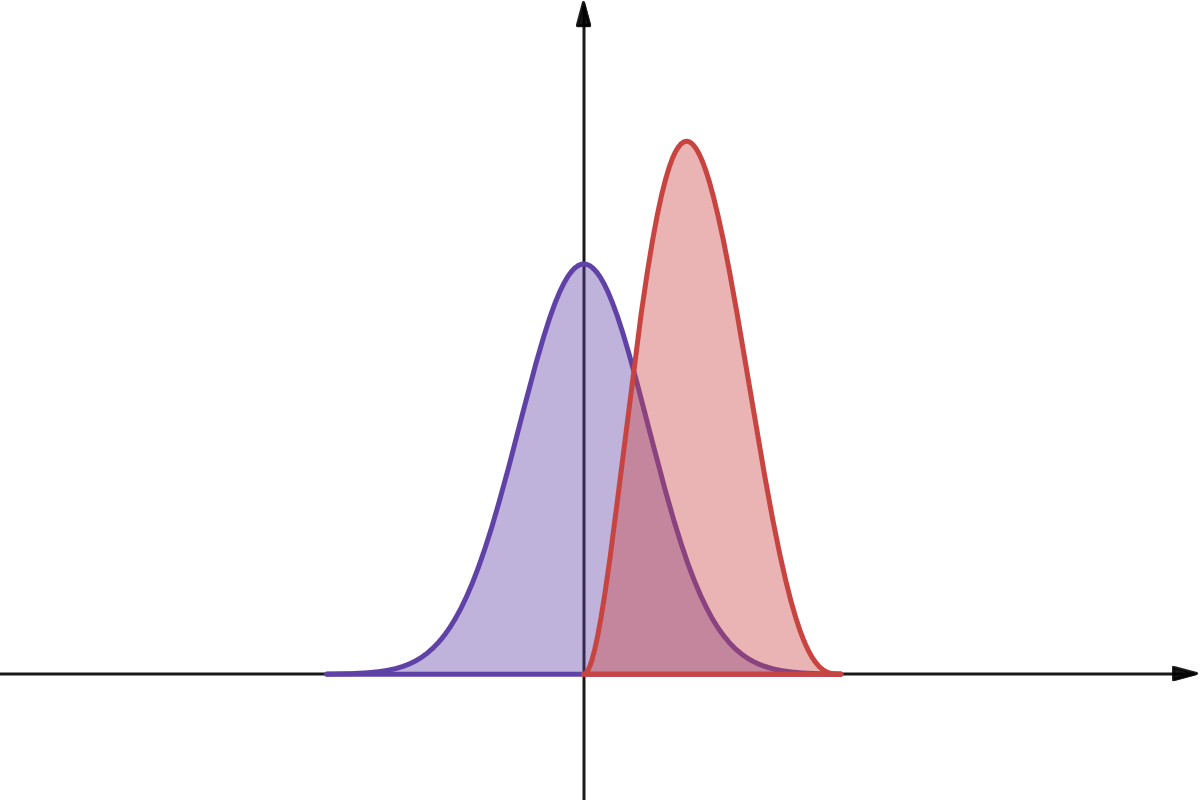
\includegraphics[width=\linewidth]{Figures/exnmodel_AB_cont.png}
	\end{subfigure} \begin{subfigure}{0.45\linewidth}
		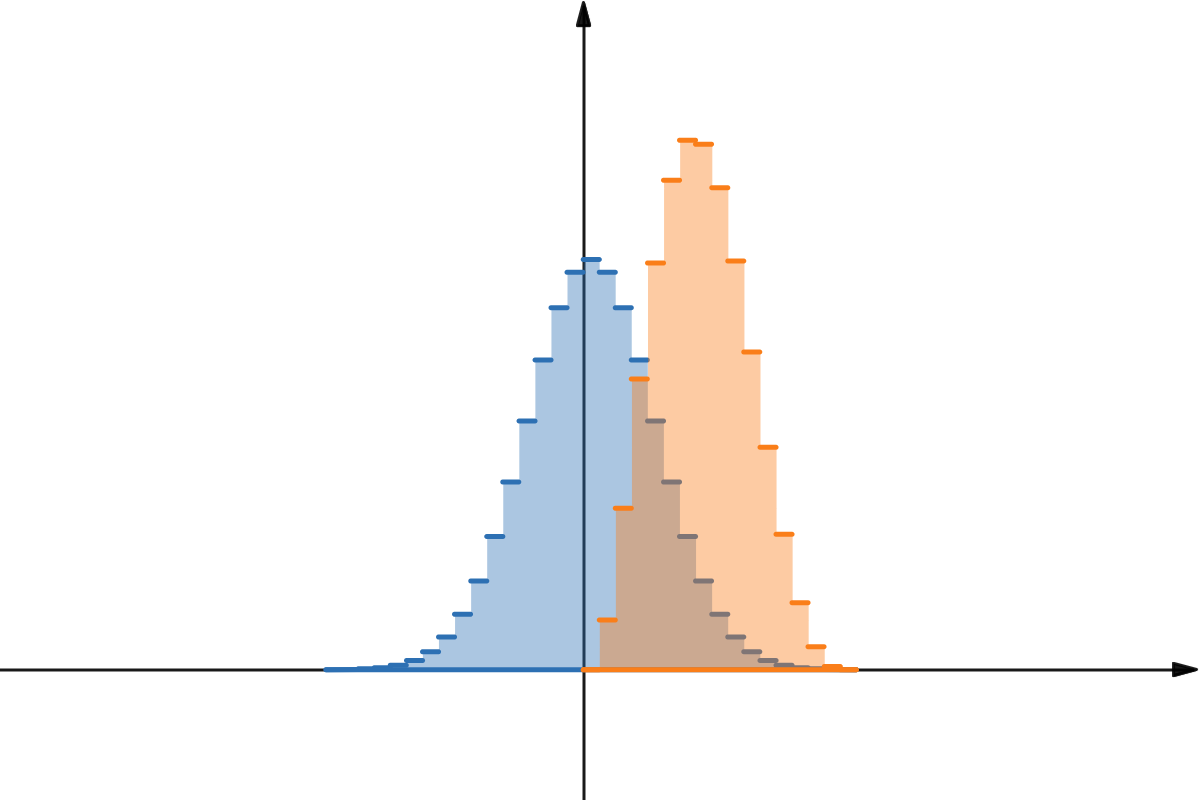
\includegraphics[width=\linewidth]{Figures/exnmodel_AB_disc.png}
	\end{subfigure}
\end{figure}

\noindent Now, let’s consider \cref{eq:SapAttribution_dist} and analyze the behavior of the estimated distance as the number of data points and the size of the boxes vary. By fixing the number of data points and decreasing the size of the boxes, the estimated distance gradually approaches $1$. This phenomenon occurs because there exists a critical dimension for $1 \;/ \; C$, such that with a sufficiently high probability, each sample becomes isolated within its own box. Consequently, this drives $J_{D_A,D_B}$ toward $0$, making each term in the summation equal to $1$.

\bigskip
In \cite{thesis}, the continuous nature of the $n$-tiles was addressed by discretizing the continuous space in which they were defined, fixing a resolution and applying posterization.\begin{toReview} Posterization is a process that reduces the number of discrete levels of color or intensity in an image, effectively mapping a continuous range of values into a smaller set of intervals. For example, in a color image, subtle variations in shades of red might all be grouped into a single pure red, removing the nuance of intermediate shades. \end{toReview} However, this approach results in a significant loss of information. Therefore, this paper will explore a method to achieve a cleaner and more dynamic discretization.

\section{Fuzzy clustering}
%La clusterizzazione fuzzy, nota anche come soft k-means, è una tecnica avanzata di analisi dei dati che consente ai punti dati di appartenere a più di un cluster. Questa modalità differisce dalla tradizionale clusterizzazione "hard", dove ogni punto dati è assegnato esclusivamente a un singolo cluster, utilizzando invece una logica fuzzy per determinare l'appartenenza di un dato a ciascun cluster. In altre parole, anziché avere un'affermazione binaria di appartenenza (1 o 0), si ha una misura continua di appartenenza che varia da 0 a 1. Questo è espresso attraverso una funzione di similarità, $\mu_x(C)$, che rappresenta il grado di appartenenza di un dato $x$ a un cluster $C$.
FFuzzy clustering, also known as soft k-means, is a data analysis technique that allows data points to be assigned to more than one cluster. Unlike traditional "hard" clustering, where each data point is assigned exclusively to a single cluster, fuzzy clustering employs fuzzy logic to determine the degree of membership for each data point within multiple clusters. Instead of a binary membership statement ($1$ or $0$), fuzzy clustering provides a continuous measure of membership that ranges from $0$ to $1$. This is represented by a similarity function, $\mu_x(C)$, which quantifies the degree to which a data point $x$ belongs to a cluster $C$.

% referenza K-Means
%La clusterizzazione fuzzy ha le sue radici nel lavoro di J.C. Dunn, che nel 1973 ha introdotto questo concetto come un'estensione dell'algoritmo di clustering k-means. Dunn ha evidenziato la maggiore precisione e robustezza della clusterizzazione fuzzy rispetto alla clusterizzazione rigida, soprattutto nella gestione dei dati anomali (outlier) \citep{FuzzyClustering_developDoc}.
\noindent Fuzzy clustering originated from the work of \citeauthor{FuzzyClustering_developDoc}, who introduced this concept as an extension of the $k$-means clustering algorithm in $1973$. \citeauthor{FuzzyClustering_developDoc} emphasized the increased accuracy and robustness of fuzzy clustering compared to hard clustering, particularly in handling anomalous data (outliers) \citep{FuzzyClustering_developDoc}.

% membership function
%L’algoritmo proposto da Dunn è detto Fuzzy C-Means Clustering (FCM) e si basa sull’utilizzo della tecnica Expectation-Maximization (EM) per definire la funzione di appartenenza ai cluster. Questa tecnica è un approccio iterativo per la stima dei parametri statistici, come ad esempio i centroidi dei cluster. Il processoEM si articola in due fasi principali:
%\begin{enumerate}
%    \item Expectation (E): In questa fase, viene formulata una funzione di verosimiglianza che esprime la probabilità che un dato appartenga a ciascun cluster in base alla sua distanza o similarità rispetto ai centroidi.
%    \item Maximization (M): Nella fase di massimizzazione, vengono individuati i parametri dei modelli che massimizzano la verosimiglianza, in questo caso i centroidi dei cluster, tramite un procedimento di ottimizzazione.
%\end{enumerate}
\noindent The algorithm proposed by \citep{FuzzyClustering_developDoc} is known as the \gls{fcm} and employs the \gls{em} technique to define the cluster membership function. This method is an iterative approach for estimating statistical parameters, such as cluster centroids. The \gls{em} process consists of two main steps:
\begin{enumerate}
    \item Expectation (E): In this phase, a likelihood function is formulated. This function expresses the probability that a data point belongs to each cluster, based on its distance or similarity to the centroids.
    \item Maximisation (M): In the maximization phase, an optimization procedure is used to identify the model parameters that maximize the likelihood, specifically the centroids of the clusters.
\end{enumerate}

%In sintesi, la clusterizzazione fuzzy offre una maggiore flessibilità rispetto alla clusterizzazione rigida, consentendo una rappresentazione più accurata e dettagliata dei dati, soprattutto in presenza di dati eterogenei o outlier.
\noindent In summary, fuzzy clustering provides greater flexibility compared to hard clustering, allowing for a more accurate and detailed representation of the data, particularly in the presence of heterogeneous data or outliers.

\subsection{Insights}
%Per comprendere appieno l'algoritmo \gls{fcm}, si definiranno preliminarmente i concetti fondamentali su cui si basa.
To fully understand the \gls{fcm} algorithm, we must first define the fundamental concepts on which it is based.

%\noindent I "punti dati" sono le osservazioni o le entità nel nostro insieme di dati, ognuna caratterizzata da una serie di attributi o feature. Questi punti dati possono essere visti come punti nello spazio multidimensionale, dove ogni dimensione corrisponde a un attributo specifico.
\noindent \textbf{Data points}: These are the observations or entities in our dataset, each characterized by a set of attributes or features. Data points can be viewed as points in a multidimensional space, where each dimension corresponds to a specific attribute.

%\noindent Una volta che abbiamo definito i punti dati, possiamo procedere a organizzarli in gruppi chiamati "cluster". Un cluster è una raccolta di punti dati che condividono caratteristiche simili tra loro. L'obiettivo dell'algoritmo di clustering è quello di raggruppare i punti dati in modo che quelli all'interno dello stesso cluster siano più simili tra loro rispetto a quelli in cluster diversi.
\noindent \textbf{Clusters}: Once we have defined the data points, we can organize them into groups called clusters. A cluster is a collection of data points that share similar characteristics. The goal of the clustering algorithm is to group data points so that those within the same cluster are more similar to each other than to those in different clusters.

%\noindent Ogni punto dati può essere associato a uno o più cluster attraverso la funzione di appartenenza a un cluster, indicata con $\mu_x$. Questa funzione assegna a ciascun punto dati un grado di partecipazione a ciascun cluster, rappresentato da un valore compreso tra $0$ e $1$. Ad esempio, se $\mu_x(C) = 1$, significa che il punto dati $x$ appartiene completamente al cluster $C$, mentre se $\mu_x(C) = 0.5$, significa che $x$ appartiene al cluster $C$ con una certa incertezza o ambiguità.
\noindent \textbf{Cluster Membership Function}: Each data point can be associated with one or more clusters through the cluster membership function, denoted as $\mu_x$, where $x$ represents a specific data point and $C$ represents a cluster. This function assigns each data point a degree of membership in each cluster, represented by a value between $0$ and $1$. For example, if $\mu_x(C) = 1$, it indicates that data point $x$ belongs completely to cluster $C$. Conversely, if $\mu_x(C) = 0.5$, it suggests that $x$ has some degree of uncertainty or ambiguity in its membership to cluster $C$.
\begin{notation}
Denote:
\begin{itemize}
\item the dataset with \\ $\mathcal{S} = (x_i)_{i=1:N}$ where $x_i\in\mathbb{R}^K$
\item the set of cluster centroids with \\ $\mathcal{C}={C_1,\dots,C_M}$ where $C_j\in\mathbb{R}^K$
\item the weight matrix with \\ $U=(u_{ij})$ dove $u_{ij}=\mu_{x_i}(C_j)$
\item the quadratic Euclidean distance matrix with \\ $D^2=(d^2_{ij})$ where $d_{ij}=\|x_i-C_j\|^2$
\end{itemize}
\end{notation}

\begin{exempli_gratia}
To understand the meaning of data points and clusters, let us consider the following example:

\noindent Imagine we need to classify the apples transported by a lorry into two color categories: green and red. However, within this set, there might also be yellow apples. The $k$-means algorithm would treat a yellow apple as an anomaly compared to the red and green apples. In contrast, fuzzy clustering quantifies this anomaly by asserting that a yellow apple is a blend of red and green.

\noindent The colours of the apples can be represented in a one-dimensional space. In this space, we observe a distribution of data points showing green and red at the extremes, with yellow apples located in the center.

\noindent Clusters, in the context of fuzzy logic, are sets defined by centroids representing specific shades of colour, which are not necessarily present in the set of data points. For example, if there are red and green apples, there are actually two centroids representing specific shades of red and green, even though there are no apples with such colour shades.

\begin{center}
	
\includegraphics[width=0.5\linewidth]{Figures/apple.png}
\end{center}
\end{exempli_gratia}

\begin{remark}
	The \gls{fcm} algorithm recognizes that real-world data may contain errors or uncertainties. Instead of rigidly assigning each data point to a single cluster, it introduces a measure of uncertainty in the assignment. This approach results in assigning a fuzzy degree of membership to each point concerning each cluster, rather than relying on a binary classification.
\end{remark}

\begin{definition}[membership measure]\label{def:fuzzy}
	Given a point $x$ and a cluster $C$, the membership measure $\mu_x(C)$ is proportional to the inverse of the square of the Euclidean distance between the point $x$ and the centroid of the cluster $C$, i.e. $\frac{1}{\|x-C\|^2}$.\\ We assume that the sum of the membership measures of $x$ to all clusters in the set $\mathcal{C}$ is equal to $1$:
	$$\sum_{C\in\mathcal{C}}\mu_x(C)=1 \quad \forall x$$
	Consequently, the membership measure $u_{ij}$ of point $x_i$ to cluster $C_j$ is computed as:
	$$u_{ij} = \frac{1}{\sum_{k}\frac{d^2_{ij}}{d^2_{ik}}}$$
\end{definition}
\begin{remark}
	The \gls{kmeans} algorithm, which is based on Boolean logic, seeks to minimise the sum of the squared distances between each data point and the centroid of the cluster to which it is assigned. In other words, the goal of the \gls{kmeans} algorithm is to minimise the sum of intra-cluster variances, where the variance of a cluster is defined as the sum of the squared distances between each point in the cluster and the cluster centroid.

	\noindent Formally, the goal of the \gls{kmeans} algorithm can be expressed as:
	\begin{equation*}
		\text{argmin}_\mathcal{C}\left[\sum_{C\in\mathcal{C}}\sum_{x \in C}\|x-C\|^2\right]
	\end{equation*}
	\noindent In the case of fuzzy clustering, the membership of a point in a cluster is expressed by a fuzzy measure instead of a Boolean logic. The objective function of the \gls{kmeans} method can be rewritten equivalently with membership measures:
	\begin{equation*}
		\sum_{C\in\mathcal{C}}\sum_{x \in \mathcal{S}}\delta_x(C)\|x-C\|^2
	\end{equation*}
	where $\delta_x(C)$ represents the membership measure of point $x$ in cluster $C$. This objective function reflects the weighting of the squared distances by the membership measure of each point in the clusters.
\end{remark}
\begin{definition}[Loss function and cluster weight]
	We define the fuzzy clustering loss function from the \gls{kmeans} algorithm as follows:
	\begin{equation}
		L_\mathcal{S}(\mathcal{C}) := \sum_{C\in\mathcal{C}}p_\mathcal{S}(C) := \sum_{C\in\mathcal{C}}\sum_{x \in \mathcal{S}}\mu_x(C)^2\|x-C\|^2
		\label{eq:loss}
	\end{equation}
	where $p_\mathcal{S}(C)$ is the sum of the squared distances between the points in the cluster $C$ and its centroid. This loss function is coercive on the centroids, which means that it tends to infinity when the centroids recede to infinity, and has a finite lower bound when the centroids are bound to a compact set in the data space. For this reason we know that there is a global minimum although the uniqueness of local minima is not guaranteed.\footnote{for more about coercitive functions, see \\ \url{https://www1.mat.uniroma1.it/people/lanzara/OTT0708/Ottimizzazione0708.pdf}}
\end{definition}
\begin{remark}
	The \gls{kmeans} algorithm and fuzzy clustering via \gls{fcm} share a similar approach in updating of cluster centroids. Both algorithms aim to find the optimal position of the centroids that minimizes the loss function based on the distances between the data points and the centroids themselves.

	\noindent In the \gls{kmeans} algorithm, the process of updating centroids occurs iteratively. Initially, centroids are randomly assigned to clusters. Data points are then assigned to the nearest clusters (based on Euclidean distance), after which the centroids are updated by averaging the points assigned to each cluster. This process is repeated until the centroids converge to stable positions.

	\noindent Similarly, the \gls{fcm} algorithm iteratively updates both the centroids of the clusters and the cluster membership measures for the points. In each iteration, the optimal centroids for a given configuration of membership measures are determined, and vice versa, until a stable configuration is reached that minimizes the loss function defined based on the membership measures and the distances between the data points and the centroids.
\end{remark}

\bigskip
\begin{theorem}[Update formula 'M']
	\label{thm:Mupdate}
    Fixed the matrix $U$, the optimisation of \cref{eq:loss} finds its minimum in the centroids according to the following update formula:
    \begin{equation}
        C^{\texttt{new}}_j = \frac{\sum_{i=1}^Nu_{ij}^2x_{i}}{\sum_{i=1}^Nu_{ij}^2} \text{\hspace{1cm}} \forall j
    \end{equation}
	\begin{proof}
	    Fixed the matrix $U$, the loss function is differentiable, convex and coercive. Consequently, to find the global minimum of the function, it is sufficient to find the points where the gradient is null.

	    \noindent Calculating the partial derivatives of the gradient with respect to the centroids $C_j$, we obtain:
	\begin{equation*}
	    \frac{\partial}{\partial C_{j}} L_\mathcal{S}(\mathcal{C}) = \frac{\partial}{\partial C_{j}} p_\mathcal{S}(C_j) = \sum_{i=1}^N\frac{\partial}{\partial C_{j}} u_{ij}^2\|x_i-C_j\|^2 = 2\sum_{i=1}^N u_{ij}^2\left(C_{j}-x_{i}\right)
	\end{equation*}

	\noindent The gradient is null when all partial derivatives are null, which implies:
	\begin{equation*}
	    \sum_{i=1}^N u_{ij}C^{\text{new}}_{j} = \sum_{i=1}^N u_{ij}x_{i} \quad \forall j
	\end{equation*}

	\noindent Since $C^{\text{new}}_j$ does not depend on the index $i$, the thesis is proved.
	\end{proof}
\end{theorem}

\begin{remark}
	The calculation of the centroid update formula in fuzzy clustering is closely tied to the concept of parameter estimation through the maximum likelihood method. Specifically, it involves maximizing the joint density of the data and model parameters, conditional on the assignment of points to clusters.
	The density to be maximized is given by:
	\begin{equation*}
	    f_U(\mathcal{S}|\mathcal{C}) \propto \prod_{i,j}\text{exp}\left[-u_{ij}^2\frac{\|x_i-C_j\|^2}{2}\right]
	\end{equation*}
	where $f_U(\mathcal{S}|\mathcal{C})$ is the joint density of the points conditioned on the set of centroids where $u_{ij}$ is the membership measure of point $x_i$ in cluster $C_j$.

	\noindent The density of the single sample $x_i$ is:
	\begin{equation*}
	    f_U^i(x_i|\mathcal{C}) \propto \prod_{j}\text{exp}\left[-u_{ij}^2\frac{\|x_i-C_j\|^2}{2}\right]
	\end{equation*}
	where $f_U^i(x_i|\mathcal{C})$ is the density of the observed datum $x_i$ conditioned on the centroids.

	\noindent The goal is to maximise the likelihood density in order to obtain accurate estimates of the model parameters, which in the context of fuzzy clustering are represented by the cluster centroids. For this reason, the algorithm is classified as \gls{em} because the phase \verb"E" sets the densities for maximum likelihood when the matrix $U$ is defined and the phase \verb"M" solves the problem by finding the centroids that best explain the model.
\end{remark}

The \cref{alg:FuzzyClustering} computes the ideal centroids in fuzzy clustering and does not directly aim to minimise of \cref{eq:loss}, but rather to iteratively updates the centroids and membership measures until a stable configuration is reached that best represents the input data.

\begin{algorithm}[h]
\caption{Fuzzy Clustering\\
	\textsc{INPUT}\\
	$\bullet$ $\mathcal{S}$: set of data $x_1,\cdots,x_N$\\
	$\bullet$ $\mathcal{C}$: centroids $C_1,\cdots,C_j$}
\begin{algorithmic}[1]
\Procedure{FuzzyClustering}{$\mathcal{S}, \mathcal{C}$}
    \While{not reached the exit criterion}
        \State $D^2 \gets (d^2_{ij})$ with $d_{ij}=\|x_i-C_j\|^2$
        \State $U^2 \gets (u_{ij}^2)$ with $u_{ij}=\left(\sum_{k}D^2_{ij}/D^2_{ik}\right)^{-1}$
        \Comment{see \cref{thm:Mupdate}}
        \For{$j \gets 1$ to $M$}
            \State $C^\text{new}_j \gets \sum_{i=1}^N x_iU^2_{ij} / \sum_{i=1}^N U^2_{ij}$
        \EndFor
    \EndWhile
\EndProcedure
\end{algorithmic}
\label{alg:FuzzyClustering}
\end{algorithm}

\subsection{Implications}
This algorithm is particularly effective for clustering problems that involve noise. Two other well-known methods operate on different paradigms: \gls{kmeans} and \gls{gmm}.

\paragraph{\gls{kmeans}} is a fundamental clustering algorithm that partitions data points into disjoint groups, where the centroids represent the mean of each group. Its primary goal is to minimize the sum of variances within these groups, resulting in well-defined clusters.

\paragraph{\gls{gmm}} is a more sophisticated algorithm based on the assumption that the data points are generated by a specific statistical process:
\begin{itemize}
    \item[1] Select with probability $p_j$ the $j$-th cluster.
    \item[2] Generate a random data point from $\mathcal{N}(C_j, \Sigma_j)$.
\end{itemize}
This method not only tries to find clusters and label data points, but also proposes normal distributions with averages $\mathcal{C}$ and covariances $\Sigma$, assigning probabilities indicating the weight of each cluster. It is possible to label the data points using the Mahalanobis distance\footnote{For more information on the Mahalanobis distance, see \url{https://en.wikipedia.org/wiki/Mahalanobis_distance}}.

\bigskip
Next, lets see how these methods behave in the presence of noisy data. Specifically, $6$ random centroids were chosen in a two-dimensional space, from which $20$, $20$, $20$, $30$, $30$ and $40$ data points with different covariance matrices were generated, respectively. In addition, uniformly generated noisy data points were added, constituting $30\%$ of the total (i.e. $48$ noisy data points). A representation of this data can be seen in \cref{fig:data_true}. As can be seen, noise can create \textit{outliers}, i.e. distant points that would be better ignored to achieve good clustering.

\begin{figure}[ht]
    \centering
    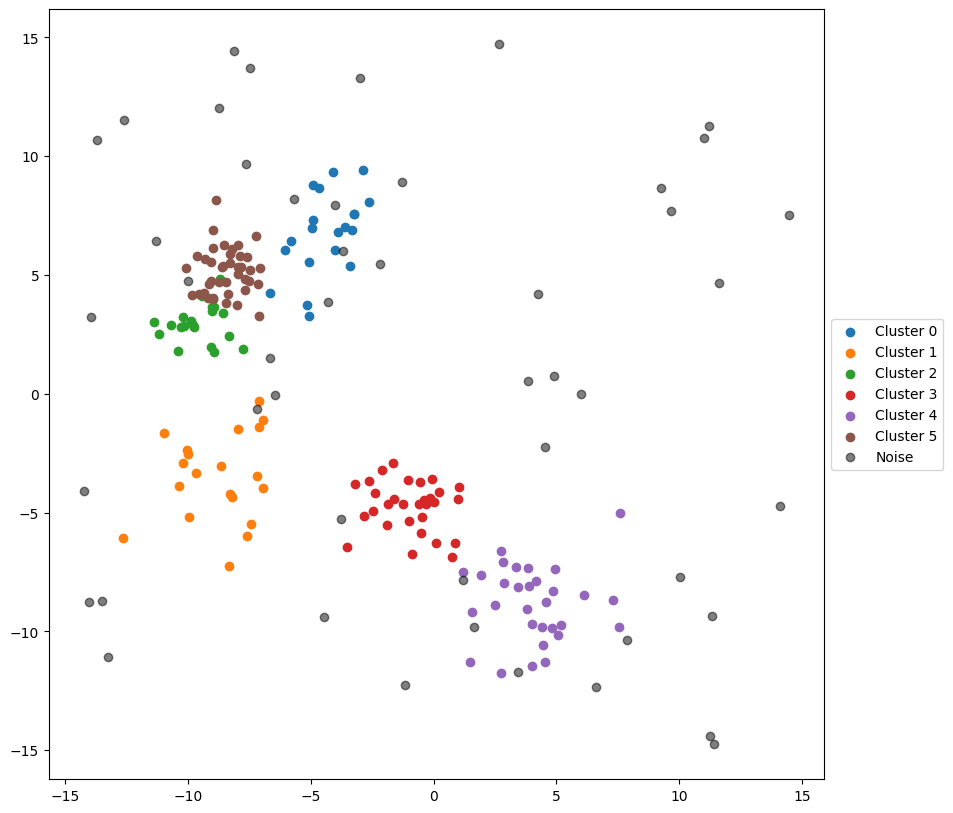
\includegraphics[width=0.9\linewidth]{Figures/dati_veri.png}
    \caption[example of data for clustering]{Data points are coloured according to their label, while noise is shown in grey.}
    \label{fig:data_true}
\end{figure}

\noindent Now let will try clustering with \gls{kmeans} using the right number of centroids, i.e. $6$. In \cref{fig:data_kmeans} we can see that the noise has created an additional cluster and two of the original clusters have merged into one. Although the result is quite satisfactory, it is not entirely clean.

\noindent Next, let is apply clustering with \gls{gmm} again using $6$ centroids. In \cref{fig:data_gmm} it can be seen that the weight of the cluster generated by the noise is very small. Furthermore, the covariance matrices allow the position of the centroids to be calculated more precisely, providing information on the nature of the clusters and creating a hierarchical structure. This is because, in reality, these are not real clusters, but normal distributions.

\noindent Finally, let clustering be applied with \gls{fcm} using $6$ centroids. In \cref{fig:data_fcm} we observe that the centroids are less affected by noise, making it possible to identify which data are potentially noisy or shared between several clusters.

\bigskip
We have observed that in the presence of noise, the algorithm \gls{fcm} can be very useful. However, the algorithm \gls{gmm}, although computationally onerous, also provides very valuable information about the nature of the data. In this thesis, we will use the \gls{fcm} algorithm to reduce the amount of information to be processed and the \gls{kmeans} algorithm for efficient initialisation of centroids.

\section{\gls{dft}}
\begin{modified}
The \gls{dft} is a powerful tool for analyzing signals in the frequency domain, often used in applications such as signal processing, image analysis, and data compression. Its ability to transform spatial or temporal data into frequency components makes it particularly effective for isolating patterns or removing noise. In this thesis, the \gls{dft} will be used to compress and clean images during the pre-processing phase, which will be discussed in detail in \cref{chap:methodology}.
\end{modified}
\begin{note}
	Nell'introduzione della tesi sarà già accennato cosa è il pre-process a grandi linee. Poi in methodology sarà descritto meglio
\end{note}

\noindent This procedure, known as spectral analysis, makes it possible to study signals, waves, vibrations, sounds and images. In addition to these areas, DFT also has major scientific applications, such as the precise estimation of sunspot cycles, helping to predict and control phenomena such as geomagnetic storms\footnote{For more about geomagnetic storms and them correlation with sunspot, see \url{https://en.wikipedia.org/wiki/Geomagnetic_storm}}.

\subsection{Insights}
\begin{modified}
	The \gls{dft} is a discrete analogue of the \gls{cft}, which represents a function in terms of its frequency components. More rigorously, given a function $f\in L^1(\mathbb{R})$, its Fourier transform is a functional operator, denoted by $\mathcal{F}$, which associates $f$ with its frequency representation:
	\[
		\mathcal{F}(f): \omega \mapsto \int_{\mathbb{R}} e^{-i2\pi \omega x}f(x)\,dx
	\]
	\begin{note}
		La periodicità di $f$ è richiesta solo nelle serie?
	\end{note}

	\noindent By contrast, the Fourier series applies specifically to periodic functions, representing them as an infinite sum of sine and cosine waves with discrete frequencies. In this context, the \gls{dft} can be viewed as a finite approximation of the Fourier series, applied to sampled data over a finite interval.
\end{modified}

\noindent The \textbf{Fourier inversion theorem} states that, if both $f$ and $\mathcal{F}(f)$ belong to $L^1(\mathbb{R})$ (i.e. they are both integrable), then for almost any $x\in\mathbb{R}$ it is possible to recover $f(x)$ via the following inverse relation:
\[
f(x)=\int_{\mathbb{R}}{\mathcal{F}\left(f\right)}(\omega)e^{i2\pi x\omega}\,d\omega
\]
In other words, the Fourier transform and its inverse allow switching back and forth between the time (or space) and frequency domains.

\bigskip
The discrete version of this transform, namely \gls{dft}, is used to analyse signals sampled at regular intervals. Thus, while \gls{cft} works on continuous signals, \gls{dft} applies to finite and discrete signals, making it suitable for digital signal processing.

\noindent To better understand how \gls{dft} gives information about the amplitudes and phases of the different frequencies that make up a sequence, it is useful to introduce the Fourier coefficients. These coefficients make it possible to decompose a data sequence into sinusoids associated with different frequencies.

\begin{modified}
\begin{remark}
	The Fourier coefficients of the sequence $(x_n)_{n=0}^{N-1}$ is a sequence of complex numbers $(X_k)_{k=0}^{N-1}$ such that:
	\begin{equation}
		x_n = \frac{1}{N}\sum_{k=0}^{N-1} X_k e^{i2\pi\frac{k}{N}n}
	\end{equation}

	\noindent In the follow examples, we want show an intuitive relation between Fourier coefficients and them time series. It is very important to interpretate a result of a \gls{dft}.
\end{remark}
\end{modified}

\begin{exempli_gratia}[Amplitude]
	\begin{toReview}
		In this example we understand how the Fourier coefficients determine the amplitude of a frequency.
	\end{toReview}

	\noindent Take a time series consisting of $N$ complex numbers, described by the following coefficients:
	\[
		X_0=0,\;X_1=A,\;X_2=0\;\cdots\;X_{N-2}=0,\;X_{N-1}=A
	\]
	From these coefficients we obtain the time series:
	\[
		x_n = \frac{1}{N}A\left(e^{i2\pi \frac{n}{N}} + e^{i2\pi \frac{n}{N}(N-1)}\right) = \frac{2A}{N}\cos\left(2\pi\frac{n}{N}\right)
	\]
	\begin{modified}
	We note that the series is only a sinusoidal function, with amplitude $\frac{2A}{N}$ and frequency $\frac{2\pi}{N}$.
	\begin{center}
		\centering
		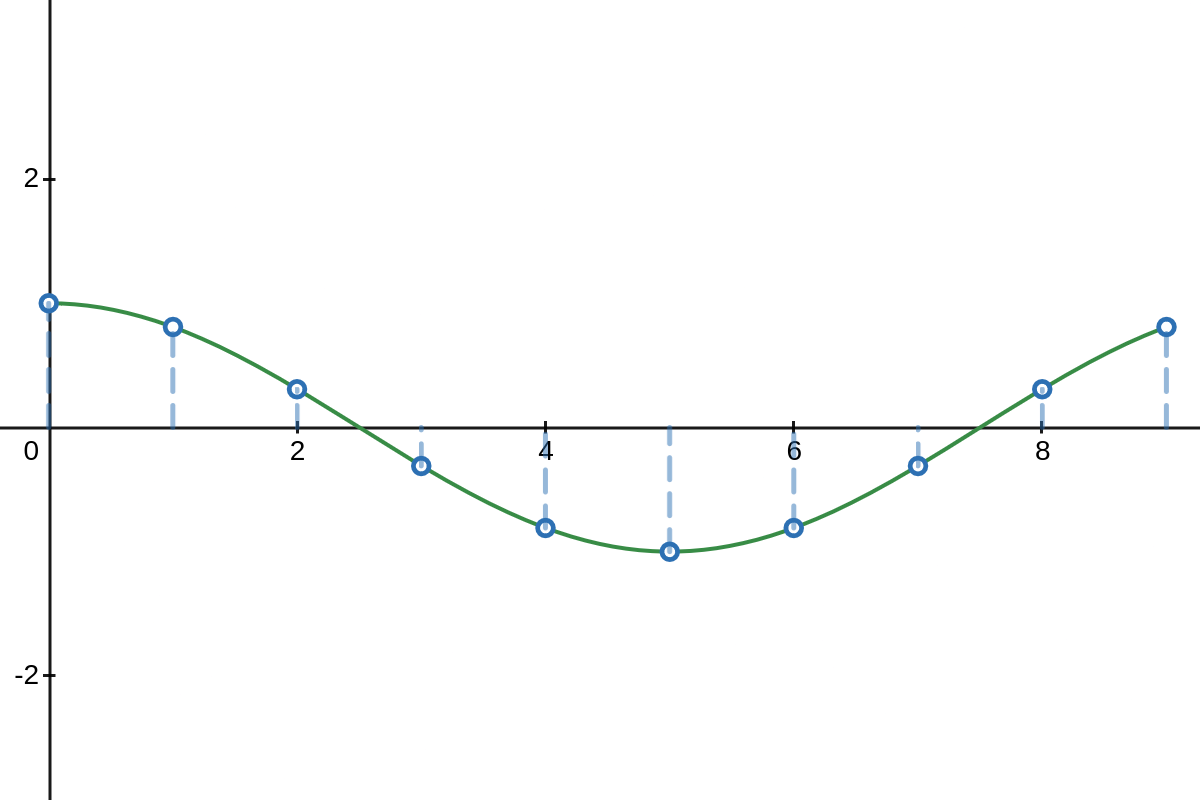
\includegraphics[width=0.5\textwidth]{Figures/fftexample1.png}
	\end{center}
	\end{modified}
\end{exempli_gratia}

\begin{exempli_gratia}[Frequency]
	\begin{toReview}
		In the previous example the significant frequency is $2\pi\frac{n}{N}$, in this example we study how to refer to a different frequency.
	\end{toReview}

	\noindent Take a time series consisting of $N$ complex numbers, described by the following coefficients:
	\[
		X_p=A,\;X_{N-p}=A
	\]
	where all other values are zero.

	\noindent The generated time series will be:
    \[
		x_n = \frac{1}{N}A\left(e^{i2\pi \frac{n}{N}p} + e^{i2\pi \frac{n}{N}(N-p)}\right) = \frac{2A}{N}\cos\left(2\pi\frac{n}{N}p\right)
	\]
	\begin{modified}
	As can be seen, the coefficients refer to the amplitude of a certain frequency indicated by the index of Fourier coefficient.
	\begin{center}
		\centering
		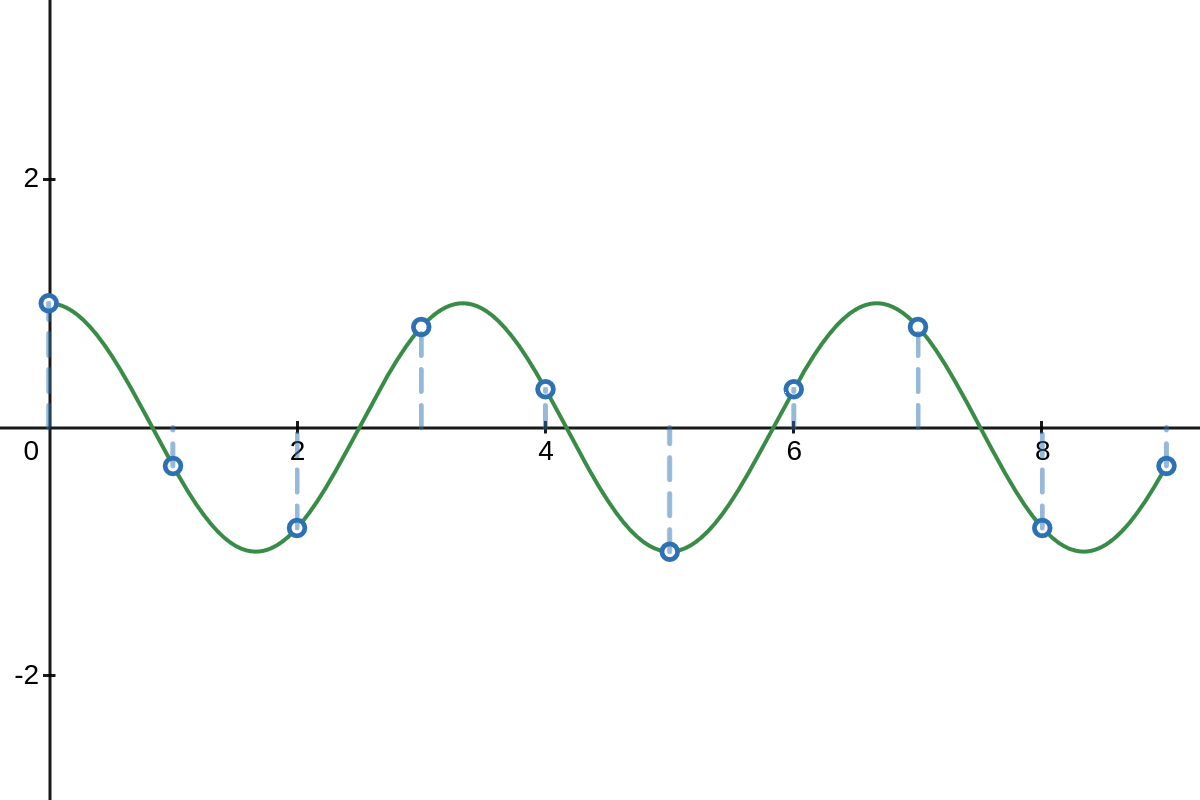
\includegraphics[width=0.5\textwidth]{Figures/fftexample2.png}
	\end{center}

	\noindent If we have $X_1=A, X_{N-1}=A$, $X_2=B, X_{N-2}=B$, then we will obtain time series:
	\[
		x_n = \frac{2A}{N}\cos\left(2\pi\frac{n}{N}\right) + \frac{2B}{N}\cos\left(2\pi\frac{n}{N}2\right)
	\]
	\end{modified}
\end{exempli_gratia}
\begin{exempli_gratia}[Phase]
	\begin{toReview}
		In the previous example we observed that the index of the Fourier coefficient refers to a specific frequency. Now we are going to see how the Fourier coefficients derive the phase of a frequency in a time series.
	\end{toReview}

	\noindent Take a time series consisting of $N$ complex numbers, described by the following coefficients:
	\[
		X_0=0,\;X_1=Ae^{i\theta},\;X_2=0,\;\dots,\;X_{N-2}=0,\;X_{N-1}=Ae^{-i\theta}
	\]
	The resulting time series will be:
    \[
		x_n = \frac{2A}{N}\cos\left(\frac{2\pi}{N}n + \theta\right)
	\]
	Here, the modulus of the coefficient describes the amplitude of the frequency, while its argument $\theta$ describes its phase.
	\begin{center}
		\centering
		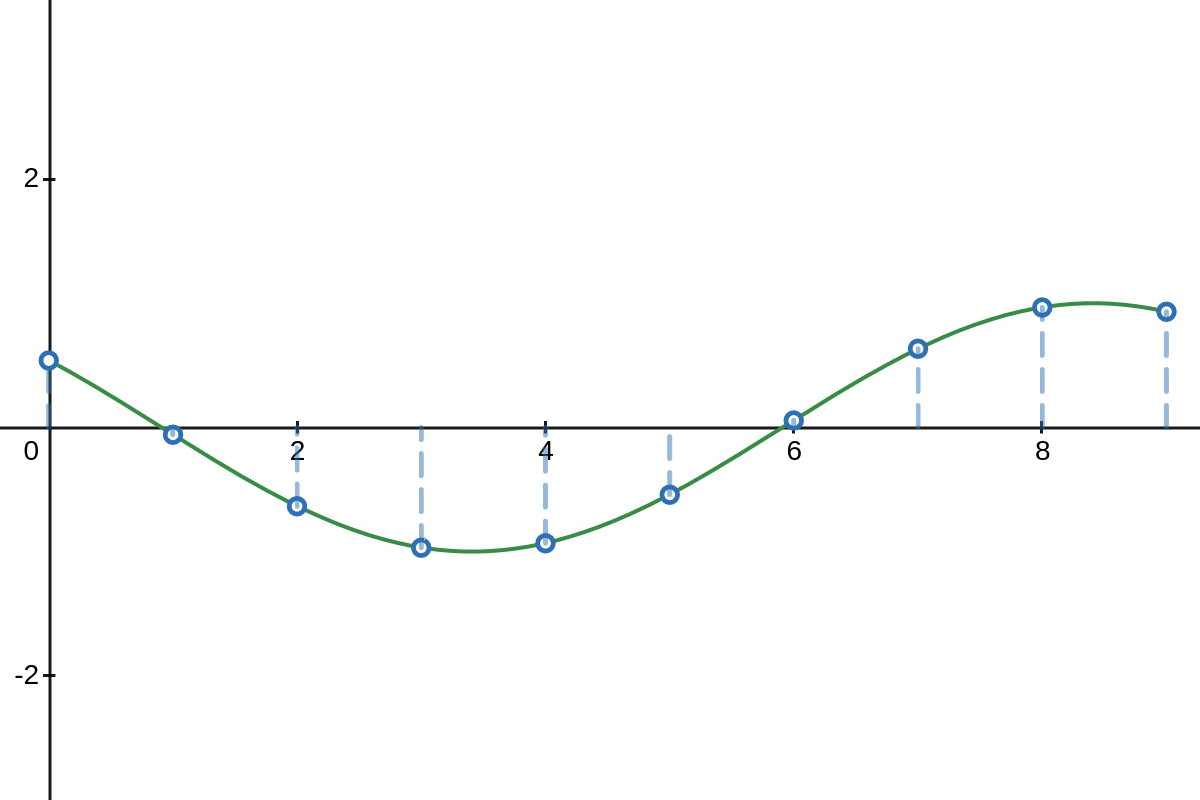
\includegraphics[width=0.5\textwidth]{Figures/fftexample3.png}
	\end{center}

	\begin{modified}
		\noindent We observe also that to ensure that the series is real, the opposite coefficient must be the conjunct of $X_1$.
	\end{modified}
\end{exempli_gratia}

\bigskip
We now ask ourselves whether it is possible to estimate the Fourier coefficients from a time series.
\begin{proposition} \label{prop:dft_unitaria}
	The matrix $\frac{1}{\sqrt{N}}\left(e^{i2\pi\frac{k}{N}n}\right)_{n,k=0}^{N-1}$ is unitary.
	\begin{proof}
		\begin{modified} We prove the thesis by studying the inner product between two rows of the matrix: \end{modified}
		\[
		\frac{1}{N}\sum_{k=0}^{N-1} e^{i2\pi\frac{k}{N}n}\cdot e^{-i2\pi\frac{k}{N}m} = \frac{1}{N}\sum_{k=0}^{N-1} e^{i2\pi\frac{k}{N}(n-m)}
		\]
		If $n = m$, the result of the sum is $1$. Else if $n \neq m$, we obtain:
		\[
			\frac{1}{N}\sum_{k=0}^{N-1} e^{i2\pi\frac{k}{N}(n-m)} = \frac{1}{N}\frac{e^{i2\pi\frac{N}{N}(n-m)}-1}{e^{i2\pi\frac{1}{N}(n-m)}-1} = 0
		\]
		This proves that the matrix is unitary.
	\end{proof}
\end{proposition}

\bigskip
Proving that the matrix $\frac{1}{\sqrt{N}}(e^{i2\pi\frac{k}{N}n})_{n,k=0}^{N-1}$ is unitary is extremely relevant to the computation of Fourier coefficients.
\begin{theorem}[\gls{dft}]
	The Fourier coefficients of the time series $(x_n)_{n=0}^{N-1}$ are given by the formula:
	\begin{equation}
		X_k = \sum_{n=0}^{N-1} x_n e^{-i2\pi\frac{n}{N}k}
	\end{equation}
	\begin{proof}
		Define $U$ as matrix $\frac{1}{\sqrt{N}}(e^{i2\pi\frac{k}{N}n})_{n,k=0}^{N-1}$

		\noindent By definition of the discrete Fourier transform, we can write $\vec{X} = \frac{1}{\sqrt{N}}U\vec{x}$, where $\vec{X}$ is the vector of Fourier coefficients and $\vec{x}$ is the vector of the original time series.

		\noindent As shown in \cref{prop:dft_unitaria}, the matrix $U$ is unitary, so it admits an inverse, which is its transposed conjugate $U^H$. \\
		Therefore, we can invert the transformation and obtain:
		\[
			\vec{x} = \sqrt{N}U^H\vec{X}
		\]

		\noindent This relation allows us to get the Fourier coefficients from the time series.
	\end{proof}
\end{theorem}

\begin{definition}[Fourier coefficient]
	We define Fourier coefficient of the time series $(x_n)^{N-1}_{n=0}$ is the sequence of complex numbers $(X_k)^{N-1}_{k=0}$:
	\[
		X_k = \sum_{n=0}^{N-1} x_n e^{-i2\pi\frac{n}{N}k}
	\]
\end{definition}

\subsection{Implications}
The possibility of calculating Fourier coefficients directly by means of a simple matrix-vector product not only makes the analysis very informative, but also easily achievable.

\begin{modified}
\paragraph{\gls{fft}} The computational cost of the matrix-vector product for computing Fourier coefficients is $O(N^2)$, which is not excessive in itself. However, there are better algorithms that compute Fourier coefficients and that reduce this cost. An example is \gls{czt} algorithm of \citet{czt_source} with computational cost $O(N\log N)$. An other example is the algorithm of \citet{FFT} showed in \cref{alg:fft}, which use a technique of \textit{divide et impera} to compute Fourier coefficients.
\begin{remark}
	The \cref{alg:fft} uses an important property of \gls{fft}: when $N=N_1\times N_2$ with $N_1, N_2> 1$ we can \textit{divide} the input sequence, \textit{impera} over them and, finally, merge results to obtain the desiderate Fourier coefficients.

	\noindent Let $x=(x_i)_{i=0}^{N-1}$ a time series, we compute these Fourier coefficients:
	\begin{itemize}
		\item $X^{0}$ are the Fourier coefficients of  $\left(x_{N_2k}\right)_k$ with $N_1$ values.
		\item $X^{1}$ are the Fourier coefficients of $\left(x_{N_2k+1}\right)_k$ with $N_1$ values.
		\item $\cdots$
		\item $X^{N_2-1}$ are the Fourier coefficients of $\left(x_{N_2k+N_2-1}\right)_k$ with $N_1$ values.
	\end{itemize}
	Now we use them to compute $X$:
	\begin{align*}
		X_k &= \sum_{n=0}^{N-1} x_n e^{-i2\pi\frac{n}{N}k} = \sum_{p=0}^{N_2-1}\sum_{l} x_{N_2l+p} e^{-i2\pi\frac{N_2l+p}{N}k} \\
		&= \sum_{p=0}^{N_2-1}\sum_{l} x_{N_2l+p} e^{-i2\pi\frac{N_2l}{N}k}e^{-i2\pi\frac{p}{N}k} \\
		&= \sum_{p=0}^{N_2-1}e^{-i2\pi\frac{p}{N}k}X^p_k
	\end{align*}
	In particular, the \cref{alg:fft} uses the case of $N_2=2$ and the follow observation:
	\begin{align*}
		X_{k+N/2} &= \sum_{n=0}^{N-1} x_n e^{-i2\pi\frac{n}{N}\left({k+N/2}\right)} = \sum_{n=0}^{N-1} x_n e^{-i2\pi\frac{n}{N}k -i2\pi\frac{n}{2}} \\
		&= \sum_{l} x_{2l} e^{-i2\pi\frac{2l}{N}k -i2\pi l} + \sum_{l} x_{2l} e^{-i2\pi\frac{2l+1}{N}k -i2\pi\frac{2l+1}{2}} \\
		&= X^0_k - e^{-i2\pi\frac{1}{N}k}X^1_k
	\end{align*}
\end{remark}
\noindent The computational cost of \cref{alg:fft} is $O(N\log N)$ if the base case (when $N$ is not even, or in general is a prime) has cost $O(N\log N)$.
\end{modified}

\begin{algorithm}[h]
	\caption[\gls{fft} algorithm]{\citet{FFT} \& \gls{czt} algorithms.\\
		\begin{minipage}[t]{\linewidth}
			\textsc{INPUT}
			\begin{itemize}[noitemsep, topsep=0pt]
				\item[$x$:] time series $x_1,\dots,x_N$
			\end{itemize}
			\textsc{OUTPUT}
			\begin{itemize}[noitemsep, topsep=0pt]
				\item[$X$:] Fourier coefficients of $x$
			\end{itemize}
		\end{minipage}
	}
	\begin{algorithmic}[1]
		\Function{FFT}{$x$}
		\If{$N$ is odd} \Return $\Call{CZT}{x}$ \Comment base case
		\EndIf

		\State $\text{even} \gets \Call{FFT}{\left[x_0,x_2,\cdots,x_{N-2}\right]}$
		\State $\text{odd} \gets \Call{FFT}{\left[x_1,x_3,\cdots,x_{N-1}\right]}$

		\State $X$ is an array of size $N$

		\For{$k\in 0,\dots,\frac{N}{2}-1$}
			\State $t \gets \exp\left(-2\pi i k / N\right)\cdot \text{odd}[k]$
			\State $X[k] \gets \text{even}[k] + t$
			\State $X[k + N/2] \gets \text{even}[k] - t$
		\EndFor
		\State \Return $X$
		\EndFunction
	\end{algorithmic}
	\label{alg:fft}
\end{algorithm}

\begin{modified}
\paragraph{Periodogram} The periodogram is a practical tool that graphically represents the amplitude of the different frequencies composing a time series, providing insight into the frequency spectrum of the signal. By visualising the power associated with each frequency, it highlights the dominant components of the spectrum, making it particularly useful for distinguishing between noise and significant frequencies. This connects directly to the theory of the \gls{dft}, as the periodogram is derived from the squared modulus of the Fourier coefficients, representing the signal's energy distribution across frequencies.

\noindent To illustrate this, we apply the \gls{dft} to the \texttt{sunspots} dataset from the \gls{r} package, which contains the number of sunspots observed each month from $1749$ to $1984$. Sunspots are known to correlate with the Sun's magnetic activity, which is believed to exhibit periodic cycles. Using the periodogram, we aim to identify these cycles, particularly the dominant periodic components in the data, and evaluate their significance compared to noise.
\begin{figure}[ht]
	\centering
	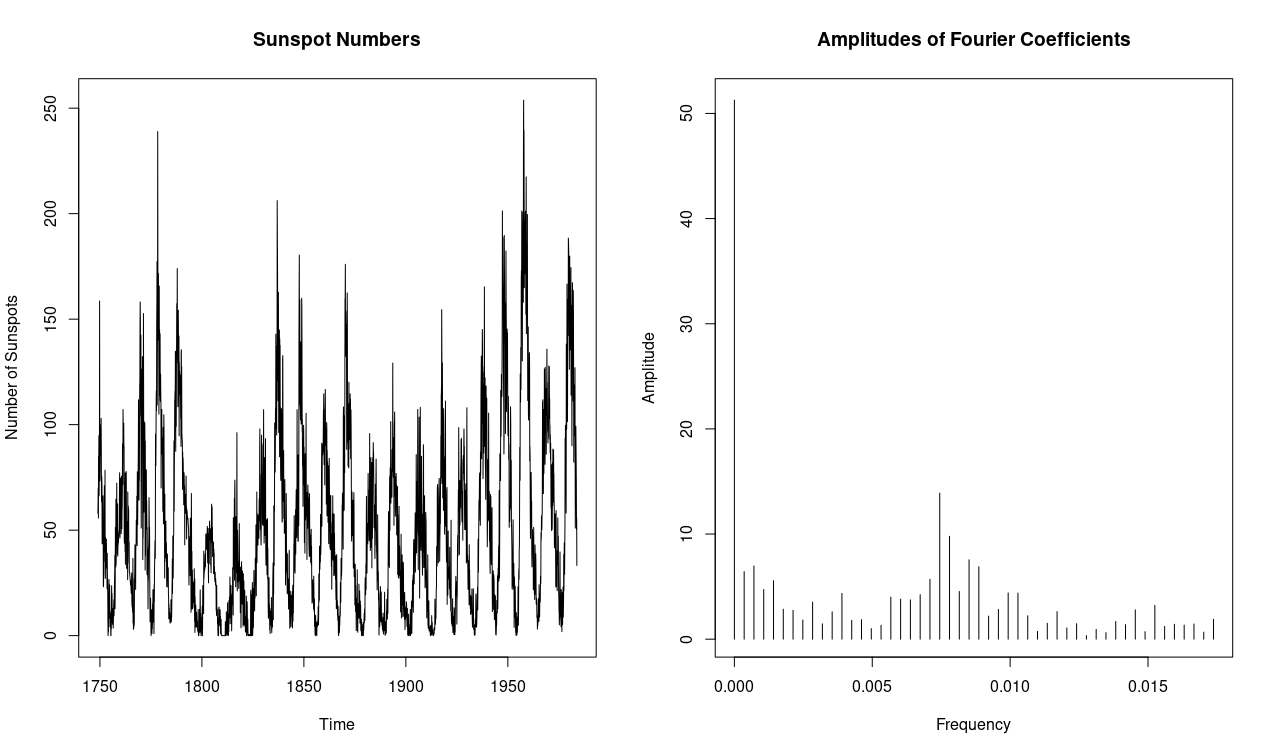
\includegraphics[width=\textwidth]{Figures/sunspots.png}
	\caption[Periodogram of sunspots]{On the left, the time series of the number of sunspots recorded each month from $1749$ to $1984$ (\(N = 2820\)). This representation shows the variation of sunspots over time, highlighting any cycles. On the right, the periodogram obtained by applying the \gls{dft} to the time series. Each point represents the squared modulus of a Fourier coefficient, which measures the energy associated with a given frequency. We can see a peak at frequency $0$, corresponding to the sum of the values of the time series (\(X_0 = \sum_{n=0}^{N-1} x_n\)).}
\end{figure}
\end{modified}

\noindent Looking at the periodogram obtained with \gls{fft}, we observe that some frequencies are much more pronounced than others. In particular, the frequency $\approx 0.0075\operatorname{\mathrm{Hz}}$ (corresponding to about a cycle of $135$ months) indicates a cycle of about $11$ years, which confirms what is already known about the cyclic nature of solar activity.

\noindent This example demonstrates how the DFT is a powerful tool for detecting and analysing periodic patterns in observational data. The use of the periodogram not only makes it possible to identify the main frequencies, but also to evaluate their relative importance respect to the background noise.

\begin{note}
	"Di qual è lo scopo della tesi mi sembra che tu non abbia parlato. Immagino ci sarà nell'introduzione? Ma in ogni caso, in apertura di questo capitolo dovresti anticipare di cosa si parlerà e perché"

	\bigskip \noindent Sì ci sarà nell'introduzione della tesi e ho messo un accenno al suo ruolo nell'introduzione della sezione DFT in queste correzioni
\end{note}

\section{Application}
\begin{modified}
In this section, we will develop specific applications of the topics discussed in this chapter to see how they can be used in the context of this thesis. The discussion will focus on the use of fuzzy clustering to address the problem of continuity in colour space, the practical implementation of the \gls{fcm} algorithm, and the use of \gls{fft} for image analysis.
\end{modified}
\subsection{Comparing works, the idea of clustering}
\begin{modified}
As we have seen, the tiles used to compute \cref{eq:SapAttribution_dist} can be represented as sequences of real numbers. However, their continuous nature introduces a problem in the computation of comparison values, since it reduces the $n$-grams to unique and unrepeatable objects (\textbf{sparsity problem}). This problem renders \cref{eq:SapAttribution_dist} ineffective, so that any pair of different works is assigned a comparison value of $1$.

\noindent One solution proposed in \cite{thesis} was the use of \textbf{posterization}, i.e., reducing the variety of colors. In this way, distinct $n$-grams could become equal after posterization, improving the comparison. However, this method introduced significant impurities and a loss of shade information.

\noindent In this thesis, a way is proposed that avoids or reduces the need for strong posterization (e.g., reduction to only two colors, \texttt{b/w}, as in \cite{thesis}). The proposed generalization is based on the dynamic use of clustering, comparing two approaches:

\begin{itemize}
	\item In \cite{thesis}: The space is clustered \textbf{a priori}, labeling the tiles with predefined boxes. The centroids take fixed values ($0$ and $1$), corresponding to the colors. For example, in the case of $1$D: the $2$-gram $(0.6, 0.8)$ will be the centroid $(1,1)$, while $(0.2, 0.8)$ will be the centroid $(0,1)$.
	\item In this thesis: The space is clustered \textbf{a posteriori}, labeling the tiles using a clustering algorithm, such as \gls{fcm}.
\end{itemize}

\noindent In this chapter, we will use \gls{kmeans}, since its application is more similar to the box system and more intuitive than \gls{fcm}. The key idea is to apply clustering on the union of tiles extracted from two works.

\noindent Doing so is expected to provide more accurate results than posterization. However, it will be necessary to provide a definition of comparative value in the case of \gls{kmeans}.
\end{modified}

\begin{exempli_gratia}[Distance between distributions reformulated with \gls{kmeans}]
	In this paragraph we will adopt the theoretically easy clustering \gls{kmeans}. Let us take $\num{10000}$ samples from $\mathcal{N}(-1,0.25)$ and $\num{40000}$ from $\mathcal{N}(+1,1)$, the two distributions will be denoted by $\mathcal{A}$ and $\mathcal{B}$ respectively.

	\begin{note}
		\noindent 32 perché sembrava graficamente meglio da vedere: 64 faceva grafici poco comprensibili e con 16 faceva dei grafici poco esplicativi. E' solo per i fini dell'esempio. (Una potenza di 2 perché per i computer è più facile gestire in memoria potenze di 2, è solo una questione mia di abitudine)
	\end{note}

	\begin{modified}
	\noindent The two sets of samples will be merged and clustered with \gls{kmeans} using $32$ centroids, resulting in a predictor $\mathcal{P}$. This predictor maps each data point $x$ to the centroid $c$ of the cluster it belongs to, i.e., $P(x)=c$ if $x$ belongs to the cluster with centroid $c$. Each cluster will be viewed as a region with a certain measure that will be the mean square of the distances of each datum in the cluster from its centroid. Given a cluster of centroid $c$, we want to estimate:
	\[
	\mu(c)=\sqrt{\mathbb{E}_{x\sim\mathcal{L}}\left[\left\|x-c\right\|^2\middle|\mathcal{P}\left(x\right)=c\right]}
	\]
	where $\mathcal{L}$ is the law of the two merged samples.

	\noindent We can see, in the image at left, that the regions has a little measure $\mu(c)$ where the density of $\mathcal{L}$ is higher. Furthermore, the image shows the weights of each cluster $c$ defined as  $\mathbb{P}_{x\sim\mathcal{L}}\left[\mathcal{P}(x)=c\right]$

	\noindent We now study the two sets of samples separately over this clustering. The densities will be weighted on the new measure $\mu$, so the density on the centroid $c$ of measure $\mu(c)$ respectively for the distribution $\mathcal{A}$ will be:
	\[
	d_\mathcal{A}(c):=\frac{p_\mathcal{A}(c)}{\mu(c)} := \frac{\mathbb{P}_{x\sim\mathcal{A}}\left[\mathcal{P}(x)=c\right]}{\mu(c)}
	\]
	similarly for $\mathcal{B}$.

	\noindent In the figure at right we show the cluster membership probabilities of the two distributions $\mathcal{A}$ and $\mathcal{B}$.

	\noindent Let us try to calculate the comparison value formulated \cref{eq:SapAttribution_dist} considering the measure:
	\begin{align*}
		d_{\gls{kmeans}}(A,B)&=(1+J_{D_A,D_B})^{-1}\frac{1}{\sum_{c\in D_A\cup D_B}\mu(c)}\sum_c \mu(c)\left(\frac{p_A(c)-p_B(c)}{p_A(c)+p_B(c)}\right)^2 \\
		&= (1+J_{D_A,D_B})^{-1}\frac{1}{\mu(D_A\cup D_B)}\int d\mu(c) \left(\frac{p_A(c)-p_B(c)}{p_A(c)+p_B(c)}\right)^2
	\end{align*}
	where $D_A$ is the support for the discretisation of ${\mathcal{A}}$ and similarly for $D_B$.\\ The result for $32$ centroids is $0.54$.

	\begin{center}
		\begin{minipage}{0.48\textwidth}
			\centering
			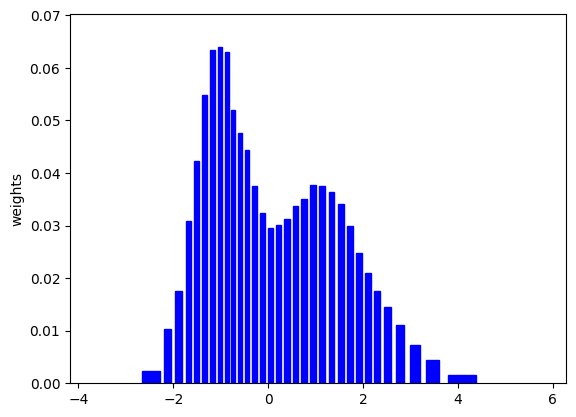
\includegraphics[width=\textwidth]{Figures/fused_analysis.png}
		\end{minipage}
		\hfill
		\begin{minipage}{0.48\textwidth}
			\centering
			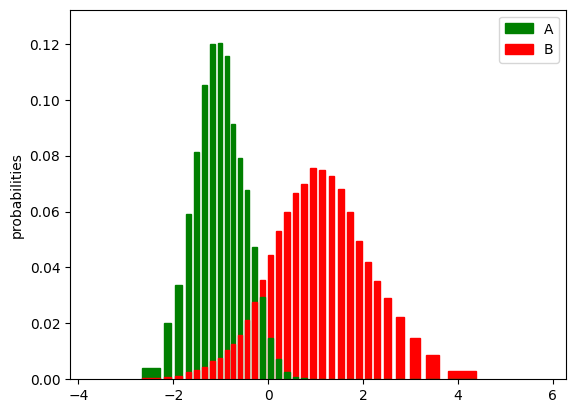
\includegraphics[width=\textwidth]{Figures/separated_analysis.png}
		\end{minipage}
	\end{center}
	\end{modified}

\end{exempli_gratia}

\begin{modified}
	In the example, an intuitive definition of a comparison value between works is proposed using clustering. In such contexts, clustering proves to be an effective tool for handling the complexity and sparsity of high-dimensional data. This is particularly relevant for counteracting the curse of dimensionality, a phenomenon where the volume of the data space is inherently vast compared to the number of available data points. In such scenarios, rigid box-based discretisations often fail because they divide the space into a fixed grid, which becomes inefficient as the dimensionality increases. The result is an exponential increase in the number of boxes, most of which remain empty or sparsely populated, leading to poor generalization.

	\noindent By contrast, dynamic clustering the data with methods such as \gls{kmeans} or \gls{fcm} allows an adaptive representation that aligns with the data distributions. Instead of imposing fixed boundaries, the centroids are positioned to capture meaningful structures in the data, improving both computational efficiency and empirical performance. This flexibility makes dynamic clustering a practical and effective choice for high-dimensional problems.
\end{modified}

\begin{toReview}
\begin{exempli_gratia}[Curse of Dimensionality]
	In this example, we compute the comparison value between the distribution \(\mathcal{N}\left(\vec{0}, \mathds{1}_\texttt{d}\right)\) in \(\mathbb{R}^K\) and itself for different values of \(K\).

	\noindent Specifically, for each \(K\), two samples \(A\) and \(B\), each containing 128 points, are taken from the same distribution. The samples are compared using two approaches: a static clustering approach (box-based) and a dynamic clustering approach (\gls{kmeans}). In the box-based method, the space is divided into \(2^K\) boxes (2 boxes per axis), while in the \gls{kmeans} method, the number of centroids is fixed at \(2\). The table below shows the average comparison values as \(K\) varies:

	\begin{minipage}{\textwidth}
		\centering
		\begin{tabular}{|>{\columncolor{pink}}c|c|c|c|c|c|}
			\hline
			Dimensions & \(1\) & \(2\) & \(4\) & \(8\) & \(16\) \\
			\hline
			Comparison with clustering & \(0.00\) & \(0.00\) & \(0.00\) & \(0.00\) & \(0.00\) \\
			\hline
			Comparison without clustering & \(0.00\) & \(0.01\) & \(0.04\) & \(0.57\) & \(1.00\) \\
			\hline
		\end{tabular}
	\end{minipage}

	\noindent Now consider two sets \(A\) and \(B\) of samples drawn from \(\mathcal{N}(\vec{0}, \mathds{1})\) and \(\mathcal{N}(\vec{1} / \sqrt{K}, \mathds{1})\) in \(\mathbb{R}^K\). These Gaussian distributions are equidistant regardless of the dimensionality \(K\), so we expect stable results. The table below reports the results of this comparison:

	\begin{minipage}{\textwidth}
		\centering
		\begin{tabular}{|>{\columncolor{pink}}c|c|c|c|c|c|}
			\hline
			Dimensions & \(1\) & \(2\) & \(4\) & \(8\) & \(16\) \\
			\hline
			Comparison with clustering & \(0.07\) & \(0.07\) & \(0.05\) & \(0.03\) & \(0.02\) \\
			\hline
			Comparison without clustering & \(0.08\) & \(0.08\) & \(0.11\) & \(0.62\) & \(1.00\) \\
			\hline
		\end{tabular}
	\end{minipage}

	\noindent The number of centroids is a critical parameter. As with boxes, too many centroids can overfit, increasing the comparison value, while too few may fail to capture the data's structure efficiently. Additionally, in high-dimensional spaces, box-based clustering becomes computationally prohibitive compared to dynamic clustering, with computation times exceeding those of \gls{kmeans} by a factor of over 100. The dynamic shape of \gls{kmeans} clusters explains this difference: a single dynamically generated cluster can cover regions spanning thousands of boxes, drastically reducing computational cost while preserving accuracy.
\end{exempli_gratia}
\end{toReview}

\subsection{Fuzzy Clustering as a Noise Filtering Method}
\begin{modified}
In this thesis, a variant of the algorithm \gls{fcm} will be used to compare two datasets. This variant introduces a weighting factor $w$, which represents the importance or contribution of each data point in the clustering process. The weight ww can be interpreted as the effective cardinality of the point: for instance, a point with $w=2$ is treated as if it were two identical points, while $w=0.5$ corresponds to half a point. This generalization allows for cleaner comparisons between sets of samples with different cardinality, simulating a balanced dataset by appropriately scaling the influence of each point.

\noindent Additionally, this variant includes specific adjustments to account for machine error in the computation of centroids (see \cref{alg:FuzzyClustering}). These adjustments improve robustness in high-dimensional spaces, with large datasets, or when using many centroids, mitigating numerical precision issues for stable clustering.
\end{modified}
\paragraph{Data's weight}
We introduce a vector $w$ indicating the weight of the data as a positive real value. As stated in \cref{thm:Mupdate,thm:Eupdate,def:fuzzyloss}, the following equations summarize the key components of the fuzzy clustering algorithm discussed so far:
\begin{align*}
	C_{j}^\text{new} &= \frac{\sum_{i=1}^N u_{ij}^2x_i}{\sum_{i=1}^N u_{ij}^2w_i} \quad \forall j\\
	L &= \sum_i\sum_j u_{ij}^2\left\|x_i-C_j\right\|^2 \\
	u_{ij} &= \frac{1}{\sum_k\frac{d_{ij}^2}{d_{ik}^2}} \quad \forall i,j\\
	d_{ij} &= \left\|x_i - C_{j}\right\| \quad \forall i,j
\end{align*}
Since it is a weighted average over $u_{ij}^2$, if a datum has a higher weight then it should increase its influence, thus having the following results:
\begin{align*}
	C_{j}^\text{new} &= \frac{\sum_{i=1}^N u_{ij}^2w_ix_i}{\sum_{i=1}^N u_{ij}^2w_i} \quad \forall j\\
	L &= \sum_i\sum_j w_{i}u_{ij}^2\left\|x_i-C_j\right\|^2 \\
	u_{ij} &= \frac{1}{\sum_k\frac{d_{ij}^2}{d_{ik}^2}} \quad \forall i,j\\
	d_{ij} &= \left\|x_i - C_{j}\right\| \quad \forall i,j
\end{align*}

\begin{note}
	Avevo scritto "pieces" perché i dati sono analizzati in batch ma questo argomento ho poi deciso di spostarlo più nelle implementazioni nel capitolo Results. Sarà rimasto come remasuio, lo tolgo...
\end{note}
\paragraph{machine error}
The use of \gls{fcm} in this thesis involves millions of data, and it is possible that the classical algorithm will find itself making serious machine errors that must be kept under control. \begin{modified} In \cref{alg:FuzzyClustering}, might exist is a value $D_{ik}^2 \approx 0$  that may be null or so small that when $D_{ij}^2 / D_{ik}^2$ is computed, it is infinity or a number so large that when added to other numbers it overshadows all other data in the sum.\end{modified}\\ For this reason \cref{alg:MembershipUpdateSafe} proposes a more robust approach. We also remark that the computational cost in a sequential algorithm will be $O(NMK)$ \marginnote{\tiny$N$ is the number of data and $M$ is the number of centroids, $K$ is the size of the tiles}. However scalability allows us to reduce this cost to $O(\text{log}(KM))$ by exploiting the independence of each cycle and scalable reductions (details in \cref{chap:methodology}).\\
\begin{note}
	In una situazione ideale dove la GPU può accettare qualsiasi livello di parallelismo, si può  lavorare sui dati indipendentemente. E usare le riduzioni (un algoritmo presentato in methodology) per abbattare i costi delle sommatorie da lineari a logaritmici.

	Poi nel capitolo results faccio notare che i limiti fisici della gpu tirano fuori un costo che comunque sarà O(NCK) ma con un fattore moltiplicativo con i dettagli hardware.
\end{note}

\begin{algorithm}[h]
\caption[Membership update stable computation.]{Membership update stable computation.\\
	\begin{minipage}[t]{\linewidth}
		\textsc{INPUT}
		\begin{itemize}[noitemsep, topsep=0pt]
			\item[$\mathcal{S}$:] set of data $x_1,\dots,x_N$
			\item[$\mathcal{C}$:] centroids $c_1,\dots,c_M$
		\end{itemize}
	\end{minipage}
}
\begin{algorithmic}[1]
\Procedure{MembershipUpdateStable}{$\mathcal{S}, \mathcal{C}$}
    \State $D^2 \gets (d^2_{ij})_{ij}$ with $d_{ij}^2=\|x_i-C_j\|^2$
    \For{$i \gets 0$ to $N$}
        \State $l \gets \min_k\{D_{ik}^2\}$
        \If{$l = 0$}
            \Where{$D_{ij}^2=0$}{$u_{ij}\gets1$}
            \Where{$D_{ij}^2\neq0$}{$u_{ij}\gets0$}
        \Else
            \State $u_{ij} \gets \frac{l}{D_{ij}^2}\quad \forall j$
        \EndIf
        \State $S_i \gets \sum_j u_{ij}$
        \State $u_{ij} \gets u_{ij} / S_i\quad\forall j$
    \EndFor
\EndProcedure
\end{algorithmic}
\label{alg:MembershipUpdateSafe}
\end{algorithm}

\subsection{Analysis of images with \gls{dft}}
It was seen in the introductory section of \gls{dft} that the algorithm \gls{fft} can only be applied to time series or, more generally, to a sequence of complex numbers. However, it is also possible to extend this concept to the analysis of the spectrum of a matrix with periodic behaviour.

\noindent Consider a matrix $x \in \mathbb{C}^{N \times M}$ defined as follows:
\[
x_{n,m} = \cos\left(\omega_rn+\omega_cm\right)
\]
It can be shown that its \gls{dft} results in a matrix of the same shape as $x$, where the only nonzero component is in the row corresponding to $\omega_r$ and in the column corresponding to $\omega_c$.

\noindent This is analogous to the application of \gls{cft} on $\mathbb{R}^2$. In particular, we would like to obtain the following inverse relation to reconstruct $x$ from its Fourier coefficients:
\begin{equation}
	x_{n,m} = \frac{1}{NM}\sum_{r,c} X_{r,c} e^{i2\pi\left(\frac{rn}{N} + \frac{cm}{M}\right)}
\end{equation}
Where the Fourier coefficients $X_{r,c}$ are given by:
\begin{equation}
	X_{r,c} = \sum_{n,m} x_{n,m}e^{-i2\pi\left(\frac{nr}{N} + \frac{mc}{M}\right)}
\end{equation}
At the algorithmic level, the two-dimensional \gls{fft} is obtained by applying the algorithm to the columns first and to the rows of the original matrix $x$. In particular:
\begin{align*}
	y_{r,m} &= \sum_{n} x_{n,m}e^{-i2\pi\frac{nr}{N}} & \;\;\text{over each column apply \gls{fft}}\\
	X_{r,c} &=\sum_{m}y_{r,m}e^{-i2\pi\frac{mc}{M}} & \;\;\text{over each row apply \gls{fft}}
\end{align*}
\begin{exempli_gratia}
	We analyse a matrix composed of several overlapping frequencies and Gaussian noise with variance $1$.
	\begin{align*}
	x_{n,m} &= 2\cos\left(2\pi(2n + 3m) + 3\right) \\
	&+ 0.8\cos\left(2\pi(n + 5m) + 2\right) \\
	&+ \cos\left(2\pi(7n + 5m)\right) + \mathcal{N}_{n,m}
	\end{align*}
	\begin{modified}
		In the figure, the original data is shown on the left as a 2D matrix visualized using the \texttt{viridis} color scale, while the Fourier coefficients computed from this matrix are displayed on the right.
	\end{modified}
	\begin{center}
		\centering 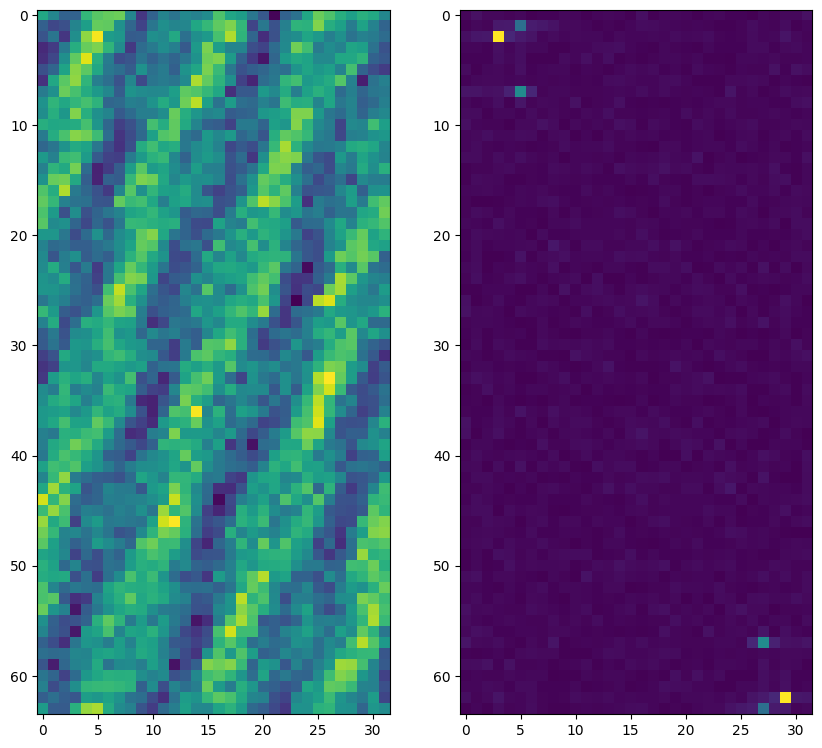
\includegraphics[width=0.6\textwidth]{Figures/fft2d_example.png}
	\end{center}
\end{exempli_gratia}

\noindent The two-dimensional \gls{fft} can be used to analyse periodic patterns in matrices that represent images or signals. Typical applications include filtering, image compression and pattern recognition, where the spectral decomposition allows significant components to be distinguished from the noise.
